\section{Formalisme Teori Permainan dan \textit{Exact Potential Game}}
Pada dasarnya, manusia tidak bisa hidup dan bekerja sendirian karena manusia sangat membutuhkan orang lain mengingat sifatnya sebagai makhluk sosial yang memiliki ketergantungan interaktif satu sama lain. Namun faktanya interaksi sosial yang dilakukan oleh manusia tidak selalu bersifat harmonis dan saling menguntungkan, melainkan sering kali terjebak dalam dilema kepentingan yang memicu persaingan strategis. Ketidakpastian hasil dari interaksi ini menuntut adanya suatu metode analisis yang mampu memetakan perilaku agen rasional dalam menghadapi skenario pilihan untuk mengoptimalkan utilitas kolektif \cite{hidalgo_quantum_2006}. Karena hal tersebut, dalam buku \textit{Theory of Games and Economic Behavior}, matematikawan John Von Neumann dan Oskar Morgenstern merumuskan formalisme matematika aksiomatik yang mengurai logika strategi di bawah kondisi ketergantungan secara sistematis \cite{john_von_neumann_theory_1953}. Paradigma ini kemudian berkembang dan memberikan landasan bagi pemodelan perilaku agen hingga tercetuslah konsep \textit{game theory} atau teori permainan yang menjadi pilar utama dalam analisis interaksi strategis \cite{galam_ising_2010}.   

\subsection{Dasar Teori Permainan Strategis dan Taksonomi Model}
Teori permainan merupakan kerangka kerja matematis aksiomatik yang digunakan untuk menganalisis interaksi strategis yang melibatkan sekumpulan agen rasional dalam lingkungan yang kompetitif. Sebuah permainan didefinisikan oleh tiga komponen fundamental yang meliputi himpunan pemain ($N$), ruang strategi ($S$), serta fungsi utilitas ($U$) bagi setiap partisipan yang terlibat. Interaksi antar pemain terjadi ketika keputusan yang diambil oleh satu agen mempengaruhi nilai utilitas atau keuntungan yang diperoleh oleh agen lainnya secara langsung, sehingga menciptakan ketergantungan yang kompleks. Terdapat berbagai fenomena interaksi strategis dalam ekosistem ekonomi yang dapat direpresentasikan secara akurat melalui model permainan klasik \cite{monderer_potential_1996}. Model permainan klasik tersebut seperti \textit{Prisoner's Dilemma}, \textit{Stag Hunt}, dan \textit{Battle of the Sexes}, menangkap esensi konflik kepentingan antar agen. Meskipun memiliki narasi konflik yang bervariasi, model-model tersebut secara formal dapat diklasifikasikan sebagai \textit{Exact Potential Game} karena memenuhi syarat penyelarasan antara utilitas marginal pemain dan perubahan fungsi potensial global \cite{monderer_potential_1996}. Dalam kerangka \textit{Prisoner's Dilemma}, pendekatan EPG memungkinkan identifikasi ekuilibrium yang stabil meskipun sering kali bersifat sub-optimal, sementara dalam \textit{Stag Hunt}, metode ini memfasilitasi penemuan titik koordinasi yang optimal bagi seluruh agen \cite{sarkar_quantum_2018}.

Ketiga model permainan tersebut memberikan kerangka \textit{benchmark} untuk memahami dinamika ekuilibrium strategis dalam sistem multi-agen dengan ketergantungan utilitas non-linear \cite{monderer_potential_1996}. Figure \ref{fig:payoffs}(a) mengilustrasikan permainan \textit{Stag Hunt} di mana strategi \textit{Stag} merepresentasikan koordinasi berisiko tinggi dengan imbal hasil maksimal, sedangkan strategi \textit{Hare} merupakan pilihan individualistik yang aman namun menghasilkan utilitas rendah bagi sistem \cite{sarkar_quantum_2018}. Dalam model \textit{Prisoner's Dilemma} yang ditunjukkan pada Figure \ref{fig:payoffs}(b), konflik muncul antara pilihan \textit{Cooperation} untuk mencapai keuntungan kolektif optimal berhadapan dengan strategi \textit{Non-cooperation} yang secara individual dominan namun berujung pada ekuilibrium yang bersifat \textit{Pareto-inferior}. Sementara itu, Figure \ref{fig:payoffs}(c) merepresentasikan \textit{Battle of the Sexes} yang mensyaratkan agen untuk melakukan koordinasi antara opsi \textit{Dog race} ($D$) dan \textit{Ballet} ($B$) meskipun terdapat preferensi imbal hasil yang asimetris di antara para pemain yang terlibat.
\begin{figure}[htbp]
    \centering
    \begin{subfigure}[b]{0.3\textwidth}
        \centering
        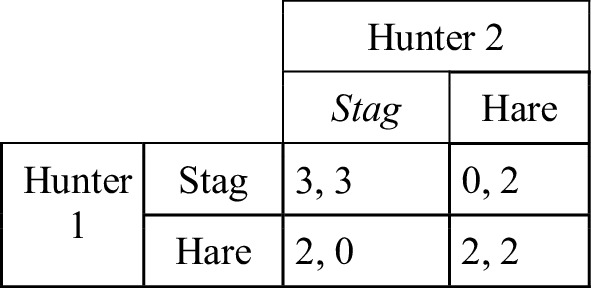
\includegraphics[width=\textwidth]{Images/payoff_SH.png}
        \caption{Stag Hunt}
        \label{fig:payoff_sh}
    \end{subfigure}
    \hfill
    \begin{subfigure}[b]{0.3\textwidth}
        \centering
        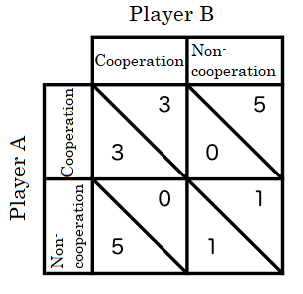
\includegraphics[width=\textwidth]{Images/payoff_PD.png}
        \caption{Prisoner's Dilemma}
        \label{fig:payoff_pd}
    \end{subfigure}
    \hfill
    \begin{subfigure}[b]{0.3\textwidth}
        \centering
        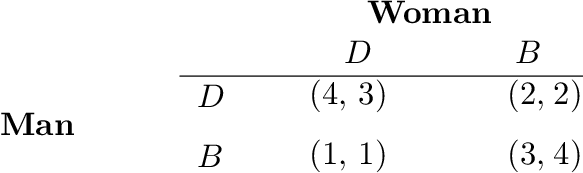
\includegraphics[width=\textwidth]{Images/payoff_BoS.png}
        \caption{Battle of the Sexes}
        \label{fig:payoff_bos}
    \end{subfigure}
    \caption{Matriks imbal hasil pada model permainan klasik: (a) \textit{Stag Hunt}, (b) \textit{Prisoner's Dilemma}, dan (c) \textit{Battle of the Sexes} yang merepresentasikan variasi struktur ekuilibrium.}
    \label{fig:payoffs}
\end{figure}
Pemetaan berbagai tipe ekuilibrium ini menjadi dasar dari berbagai kasus dalam menganalisis fenomena mikrostruktural pasar \cite{galam_ising_2010}.

\subsection{EPG \textit{Exact Potential Game} sebagai Algoritma Pencarian Ekuilibrium Nash}
Ekuilibrium Nash atau \textit{nash equilibrium} merupakan konsep stabilitas fundamental dalam teori permainan di mana tidak ada satu pun pemain yang dapat meningkatkan utilitasnya dengan mengubah strategi secara sepihak tanpa adanya perubahan dari pihak lain. Dalam sistem finansial, sebagian besar interaksi strategis antar agen ekonomi direpresentasikan melalui model permainan koordinasi (\textit{coordination game}) yang mana setara dengan struktur \textit{Stag Hunt} \cite{szabo_evolutionary_2016}. Pemilihan model ini didasarkan pada fakta bahwa pasar sangat bergantung pada sinkronisasi keputusan para investor. Kerja sama kolektif untuk mempertahankan aset memberikan imbal hasil maksimal dibandingkan pilihan individualis untuk keluar dari pasar \cite{sarkar_quantum_2018}. Namun, identifikasi titik ekuilibrium tersebut sering kali menghadapi kendala komputasi yang berat karena ruang solusi yang bersifat non-konveks serta diskrit, terutama pada sistem yang memiliki jumlah agen sangat besar.

\textit{Exact Potential Game} (EPG) hadi untuk mengatasi maslah tersebut. EPG didefinisikan sebagai kelas permainan strategis khusus di mana perubahan utilitas marginal setiap pemain selaras dengan variasi sebuah fungsi potensial global \cite{monderer_potential_1996}. Secara matematis, eksistensi fungsi potensial ($P$) menunjukkan bahwa setiap insentif agen untuk meningkatkan keuntungan lokal akan berujung pada peningkatan nilai potensial global \cite{jain_multi-portfolio_2012}. Karakteristik penyelarasan tersebut dapat menyederhanakan masalah optimasi multi-agen yang sangat kompleks menjadi masalah maksimisasi fungsi tunggal yang jauh lebih efisien untuk dikelola secara komputasional. Dalam sistem pasar finansial, EPG berfungsi sebagai algoritma pencarian ekuilibrium Nash yang andal melalui pemanfaatan mekanisme dinamika respons-terbaik (\textit{Best-Response Dynamics}) secara iteratif \cite{jain_multi-portfolio_2012}. Implementasi memiliki prosedur lewat perumusan sebuah sistem permainan dalam bentuk algoritma yang memanfaatkan variabel $\omega_n^0$ sebagai representasi bobot portofolio awal bagi setiap agen $n$ di dalam himpunan strategi layak $K_n$. Indeks $q$ digunakan untuk melacak kemajuan tahapan iteratif, di mana profil strategi kolektif $\mathbf{\omega}^q$ dievaluasi terhadap fungsi utilitas $u_n$ secara kontinu untuk mendapatkan konvergensi sistem menuju titik stabil. Mekanisme pembaruan sekuensial (Gauss-Seidel) beroperasi dengan mengintegrasikan informasi strategis terbaru dari agen sebelumnya, sementara pembaruan simultan (Jacobi) menggunakan data dari iterasi lampau untuk menghitung respon terbaik secara paralel bagi seluruh partisipan pasar. Struktur operasional algoritma iteratif tersebut dapat ditinjuau pada algoritma \ref{alg:best_response}.

\begin{algorithm}[htbp]
\caption[Iterative Best Response Algorithm]{Iterative Best Response Algorithm \cite{jain_multi-portfolio_2012}}
\label{alg:best_response}
\begin{algorithmic}[1]
\State \textbf{Data:} Pilih strategi awal $\omega_n^0 \in K_n$ untuk semua $n = 1, \dots, N$, dan set $q = 0$.
\State \textbf{Step 1:} Jika $\mathbf{\omega}^q$ memenuhi kriteria penghentian yang sesuai: \textbf{STOP}.
\State \textbf{Step 2:} Perbarui strategi $\omega_n^{q+1}$ untuk $n = 1, \dots, N$ menggunakan salah satu metode:
    \State \quad \textbf{Sequential (Gauss-Seidel) Update:}
    \State \quad $\omega_n^{q+1} \leftarrow \arg \min_{\omega_n \in K_n} u_n(\omega_1^{q+1}, \dots, \omega_{n-1}^{q+1}, \omega_n, \omega_{n+1}^q, \dots, \omega_N^q)$
    \State \quad \textbf{Simultaneous (Jacobi) Update:}
    \State \quad $\omega_n^{q+1} \leftarrow (1 - \frac{1}{N})\omega_n^q + \frac{1}{N} \cdot \arg \min_{\omega_n \in K_n} u_n(\omega_1^q, \dots, \omega_{n-1}^q, \omega_n, \omega_{n+1}^q, \dots, \omega_N^q)$
\State \textbf{Step 3:} Set $q \leftarrow q + 1$; dan kembali ke \textbf{Step 1}.
\end{algorithmic}
\end{algorithm}

\subsection{Model Markowitz dan Strategi Inisialisasi EPG}
Implementasi kerangka kerja \textit{Exact Potential Game} dalam pemilihan aset strategis dimulai dengan melakukan transformasi sistematis terhadap fungsi objektif \textit{Mean-Variance} Markowitz dari domain kontinu menuju representasi biner yang diskrit \cite{markowitz_portfolio_1952}. Proses binerisasi ini dilakukan dengan memetakan bobot portofolio ($\omega_i$) menjadi variabel keputusan $x_i \in \{0, 1\}$ melalui relasi $\omega_i = x_i / K$, di mana konstanta $K$ menyatakan jumlah total instrumen yang dipilih. Perubahan representasi ini memungkinkan masalah alokasi modal ditransformasikan menjadi pencarian konfigurasi sistem partikel yang saling berinteraksi untuk meminimalkan total konflik atau risiko di dalam portofolio investasi \cite{abdul_hali_markowitz_2020}. Formulasi fungsi biaya yang semula dinyatakan dalam bentuk Lagrangian ($\mathcal{L}$) kemudian dikonversi menjadi fungsi utilitas ($U$) yang harus dimaksimalkan oleh para agen di pasar melalui persamaan berikut:
\begin{equation}
\label{eq:lagrangian_biner}
\mathcal{L}(\mathbf{x}) = \frac{1}{K^2} \sum_{i,j} \sigma_{ij} x_i x_j - \frac{\lambda}{K} \sum_i \mu_i x_i
\end{equation}
\begin{equation}
\label{eq:utilitas_biner}
U(\mathbf{x}) = - \frac{1}{\lambda} \mathcal{L}(\mathbf{x}) = \sum_i \frac{\mu_i}{K} x_i - \frac{\gamma}{2K^2} \sum_{i,j} \sigma_{ij} x_i x_j
\end{equation}
di mana $\gamma$ merepresentasikan parameter penghindaran risiko yang berbanding terbalik dengan toleransi risiko investor.

Pembuktian koherensi model Markowitz sebagai sistem EPG bergantung pada sifat simetri dari matriks kovarians ($\sigma_{ij} = \sigma_{ji}$) yang mana mengisolasi interaksi antar aset tanpa kehilangan informasi korelasi. Fungsi potensial global ($\Phi$) didefinisikan identik dengan fungsi utilitas sistem, di mana suku-suku interaksi kuadratik dapat didekomposisi untuk mengidentifikasi kontribusi gabungan dari setiap variabel keputusan individual agen. Dengan memanfaatkan properti biner $x_i^2 = x_i$, total energi potensial sistem dapat dipisahkan menjadi komponen utilitas lokal dan insentif marginal ($\Delta \Phi$) yang eksplisit bagi setiap pemain yang terlibat \cite{monderer_potential_1996}. Insentif bagi agen untuk meningkatkan utilitas individualnya akan secara paralel meningkatkan nilai fungsi potensial global yang mencerminkan stabilitas portofolio melalui relasi
\begin{equation}
\label{eq:insentif_marginal}
\Delta \Phi = \Phi(1, \mathbf{x}_{-i}) - \Phi(0, \mathbf{x}_{-i}) = \frac{\mu_i}{K} - \frac{\gamma \sigma_{ii}}{2K^2} - \frac{\gamma}{K^2} \sum_{j \neq i} \sigma_{ij} x_j.
\end{equation}
Ekuilibrium Nash akan tercapai ketika tidak ada satu pun agen yang memiliki insentif positif ($\Delta \Phi > 0$) untuk mengubah status keputusannya secara sepihak di dalam ekosistem pasar modal. Konfigurasi yang diperoleh dari kerangka EPG ini kemudian dimanfaatkan sebagai tebakan awal (\textit{warm start}) untuk memandu proses optimasi pada tahap komputasi kuantum selanjutnya \cite{jain_multi-portfolio_2012}. Penggunaan inisialisasi berbasis EPG sangat krusial untuk mencegah algoritma variasi kuantum (yang akan dijelaskan pada bab \S\ref{sec:algoritma-vqe}) terjebak dalam fenomena \textit{local minima} atau \textit{Barren Plateaus} \cite{mcclean_barren_2018}. 